%************************************************
\chapter{Self-Test}
%************************************************
\begin{flushright}
April 8, 2013
\end{flushright}
\section{Aim}
To separate the following mixtures, using any suitable technique:
\begin{enumerate}
	\item Mixture 1: Phenol and Aniline
	\item Mixture 2: Benzoic Acid and Naphthalene
\end{enumerate}

\section {Chemicals Required}
	Aside from the mixtures provided, we required the chemicals used in \autoref{solventExtraction} viz.
	\begin{enumerate}
		\item Silica
		\item Iodine
		\item Ethyl Acetate
		\item Benzene
		\item $NaHCO_3$ saturated solution
		\item $HCl$ 6N
	\end{enumerate}	

\section{Theory}
	The first set of compounds (mixture 1) could be separated directly using the method used in \autoref{solventExtraction} for Phenol and Napthol are chemically very similar. The idea is to selectively dissolve Naphthol in a polar solvent by using a base (aqueous), leaving Aniline in the organic phase (in this case, Ethyl Acetate). Then the aqueous medium is neutralized and Naphthol recovered in an organic phase which completes the separation.
	\par
	For mixture 2, Benzoic Acid was selectively dissolved in the Sodium Bicarbonate solution. Naphthalene was filtered out and the solution neutralized. The Acid could then be recovered by crystallization.
\section{Procedure}
	Procedure for the first part is identical to that given in \autoref{solventExtraction}. It has been reproduced here for clarity (with minor adaptations).
	\begin{enumerate}
		\item The volume of the given mixture was increased by adding Ethyl Acetate (the solvent).
		\item The given mixture was taken in a separating funnel (after ensuring it's clean of course)
		\item To the mixture $NaHCO_3$ was added and the funnel shaken well
		\item The two layers were allowed to separate
		\item The bottom layer was extracted in a beaker
		\item Again $NaHCO_3$ was added and the procedure repeated
		\item The organic layer should now contain only Aniline; This was confirmed by running a TLC
		\item The contents of the beaker were neutralized using a pH paper and $HCl$
		\item The content of the beaker was transferred into the separating funnel again and Ethyl Acetate was added, shaken
		\item Both layers were collected in separate beakers and the aqueous layer was again put into the separating funnel, and the process repeated
		\item The organic layer extracted should contain only Phenol; This was confirmed by running a TLC
	\end{enumerate}
	\par
	For the second part, 
	\begin{enumerate}
		\item The given mixture (which was a solid) was dissolved in Sodium Bicarbonate
		\par
			\emph{only Benzoic Acid reacted and Naphthalene was left unreacted}
		\item The filtrate was removed using a filter paper and dried
		\item It was then dissolved in hexane and was tested for purity using TLC.
		\item The solution obtained after filtering was neutralized using pH paper and HCl
		\item TLC for the same was tested
		\item Crystallization/Extraction could be carried out to obtain Benzoic Acid (but couldn't be done successfully in the given constraints)
	\end{enumerate}
	% Benzoic Acid, $NaHCO_3$, filtered Napthalene. crystallization couldn't be carried out successfully.

\section{Observations and Results}
	Both the mixtures were separated into their corresponding components in accordance with the methods described. Benzoic Acid wasn't successfully purified however. 
	\par
	For Mixture 1, TLC for Aniline is given in \autoref{e11_aniline}, and the same for Phenol is given in \autoref{e11_phenol}
	\par
	For Mixture 2, TLC for the mixture is given in \autoref{e11_mixB}, for Benzoic Acid in \autoref{e11_benzoic} and for Naphthalene in \autoref{e11_naphthalene}.
	\par
	(Calculation of $R_f$ values has been omitted for there were only two known compounds and on the basis of polarity, the spots can be identified with the compounds.)
	\begin{figure}[bth]
		\begin{center}
			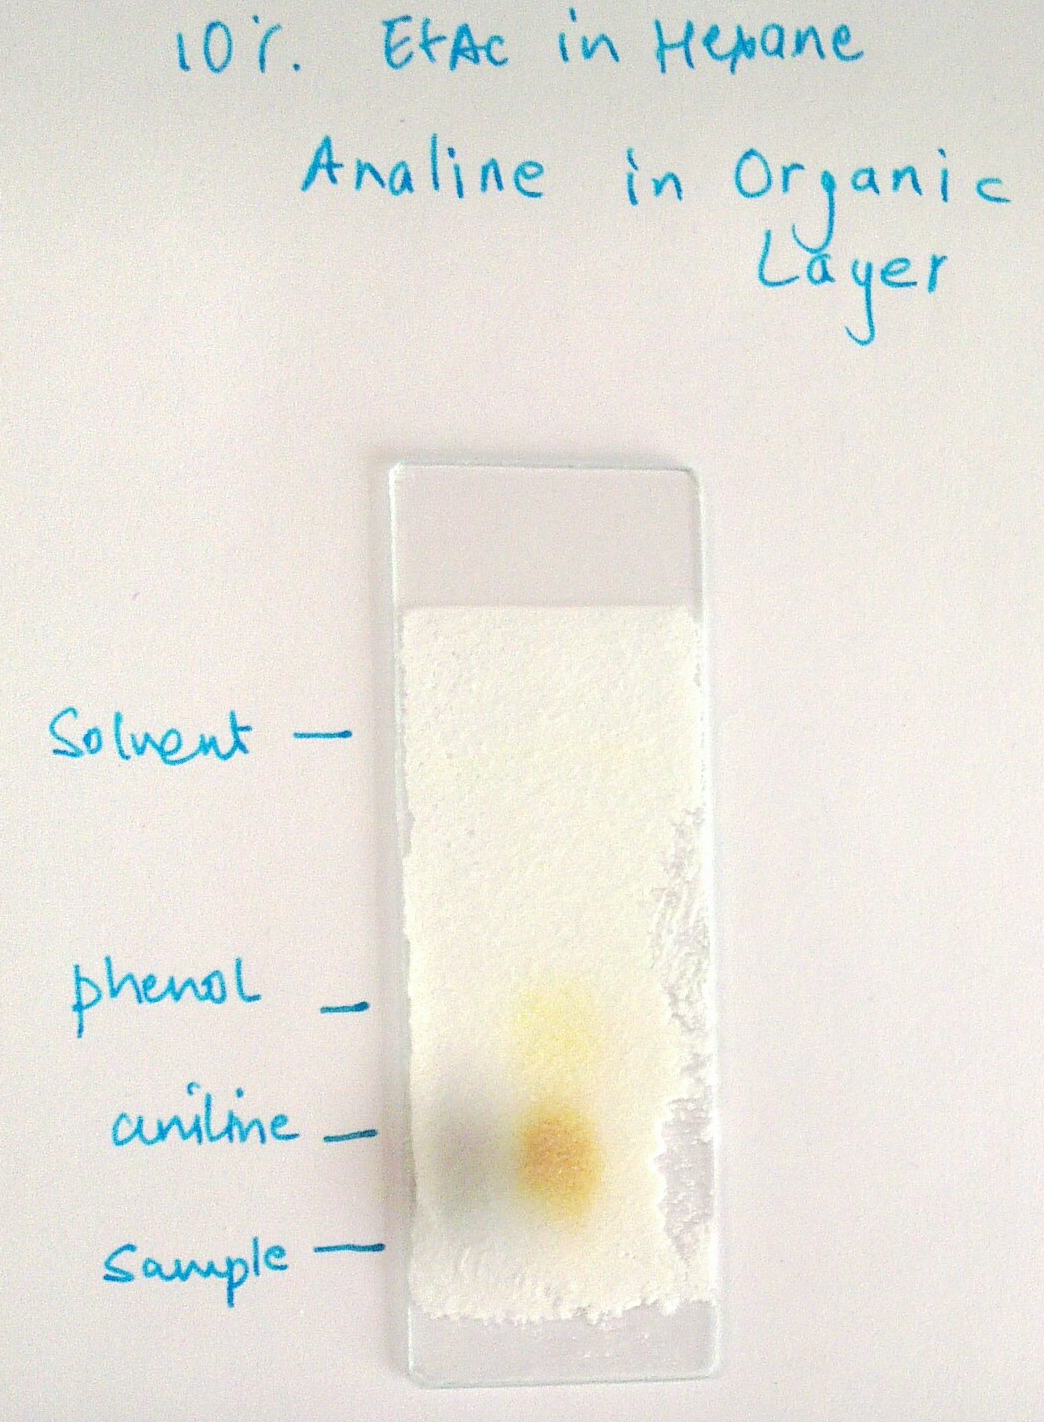
\includegraphics[width=0.4\linewidth]{gfx/e11_aniline}
		\end{center}
	\caption[TLC for Aniline]{Aniline} {\label{e11_aniline}}
	\end{figure}

	\begin{figure}[bth]
		\begin{center}
			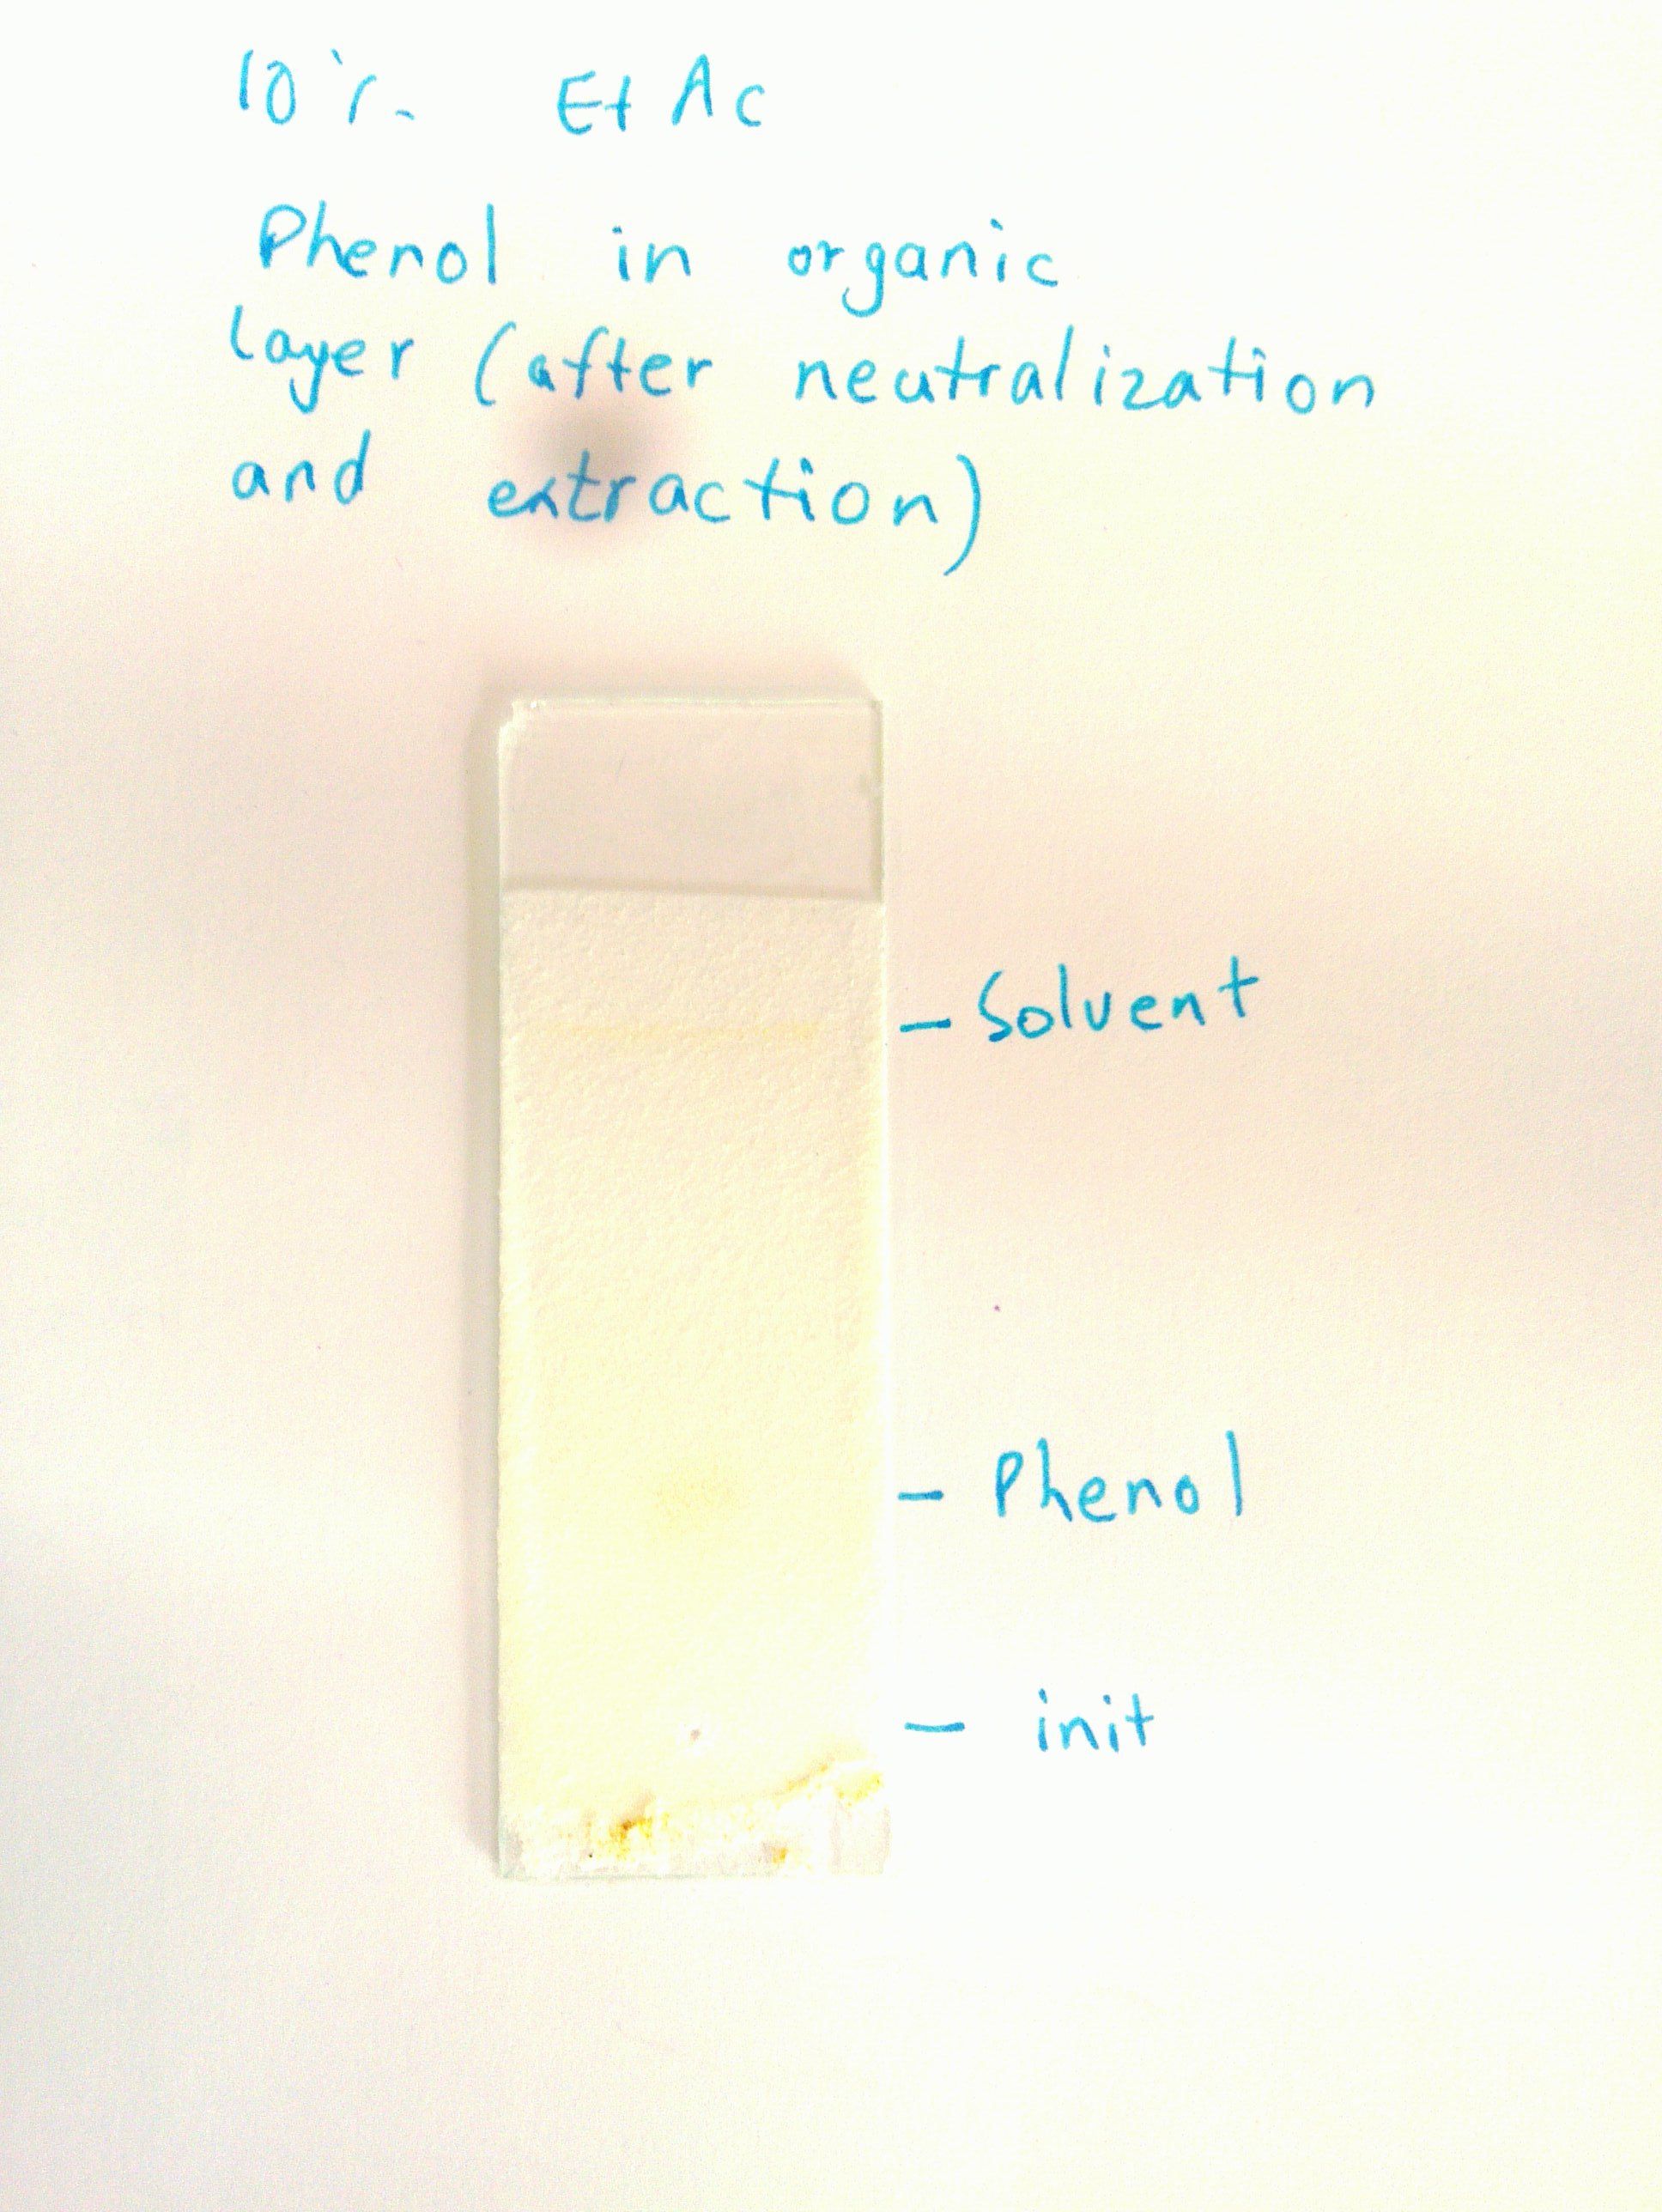
\includegraphics[width=0.4\linewidth]{gfx/e11_phenol}
		\end{center}
	\caption[TLC for Phenol]{Phenol} {\label{e11_phenol}}
	\end{figure}
	

	\begin{figure}[bth]
		\begin{center}
			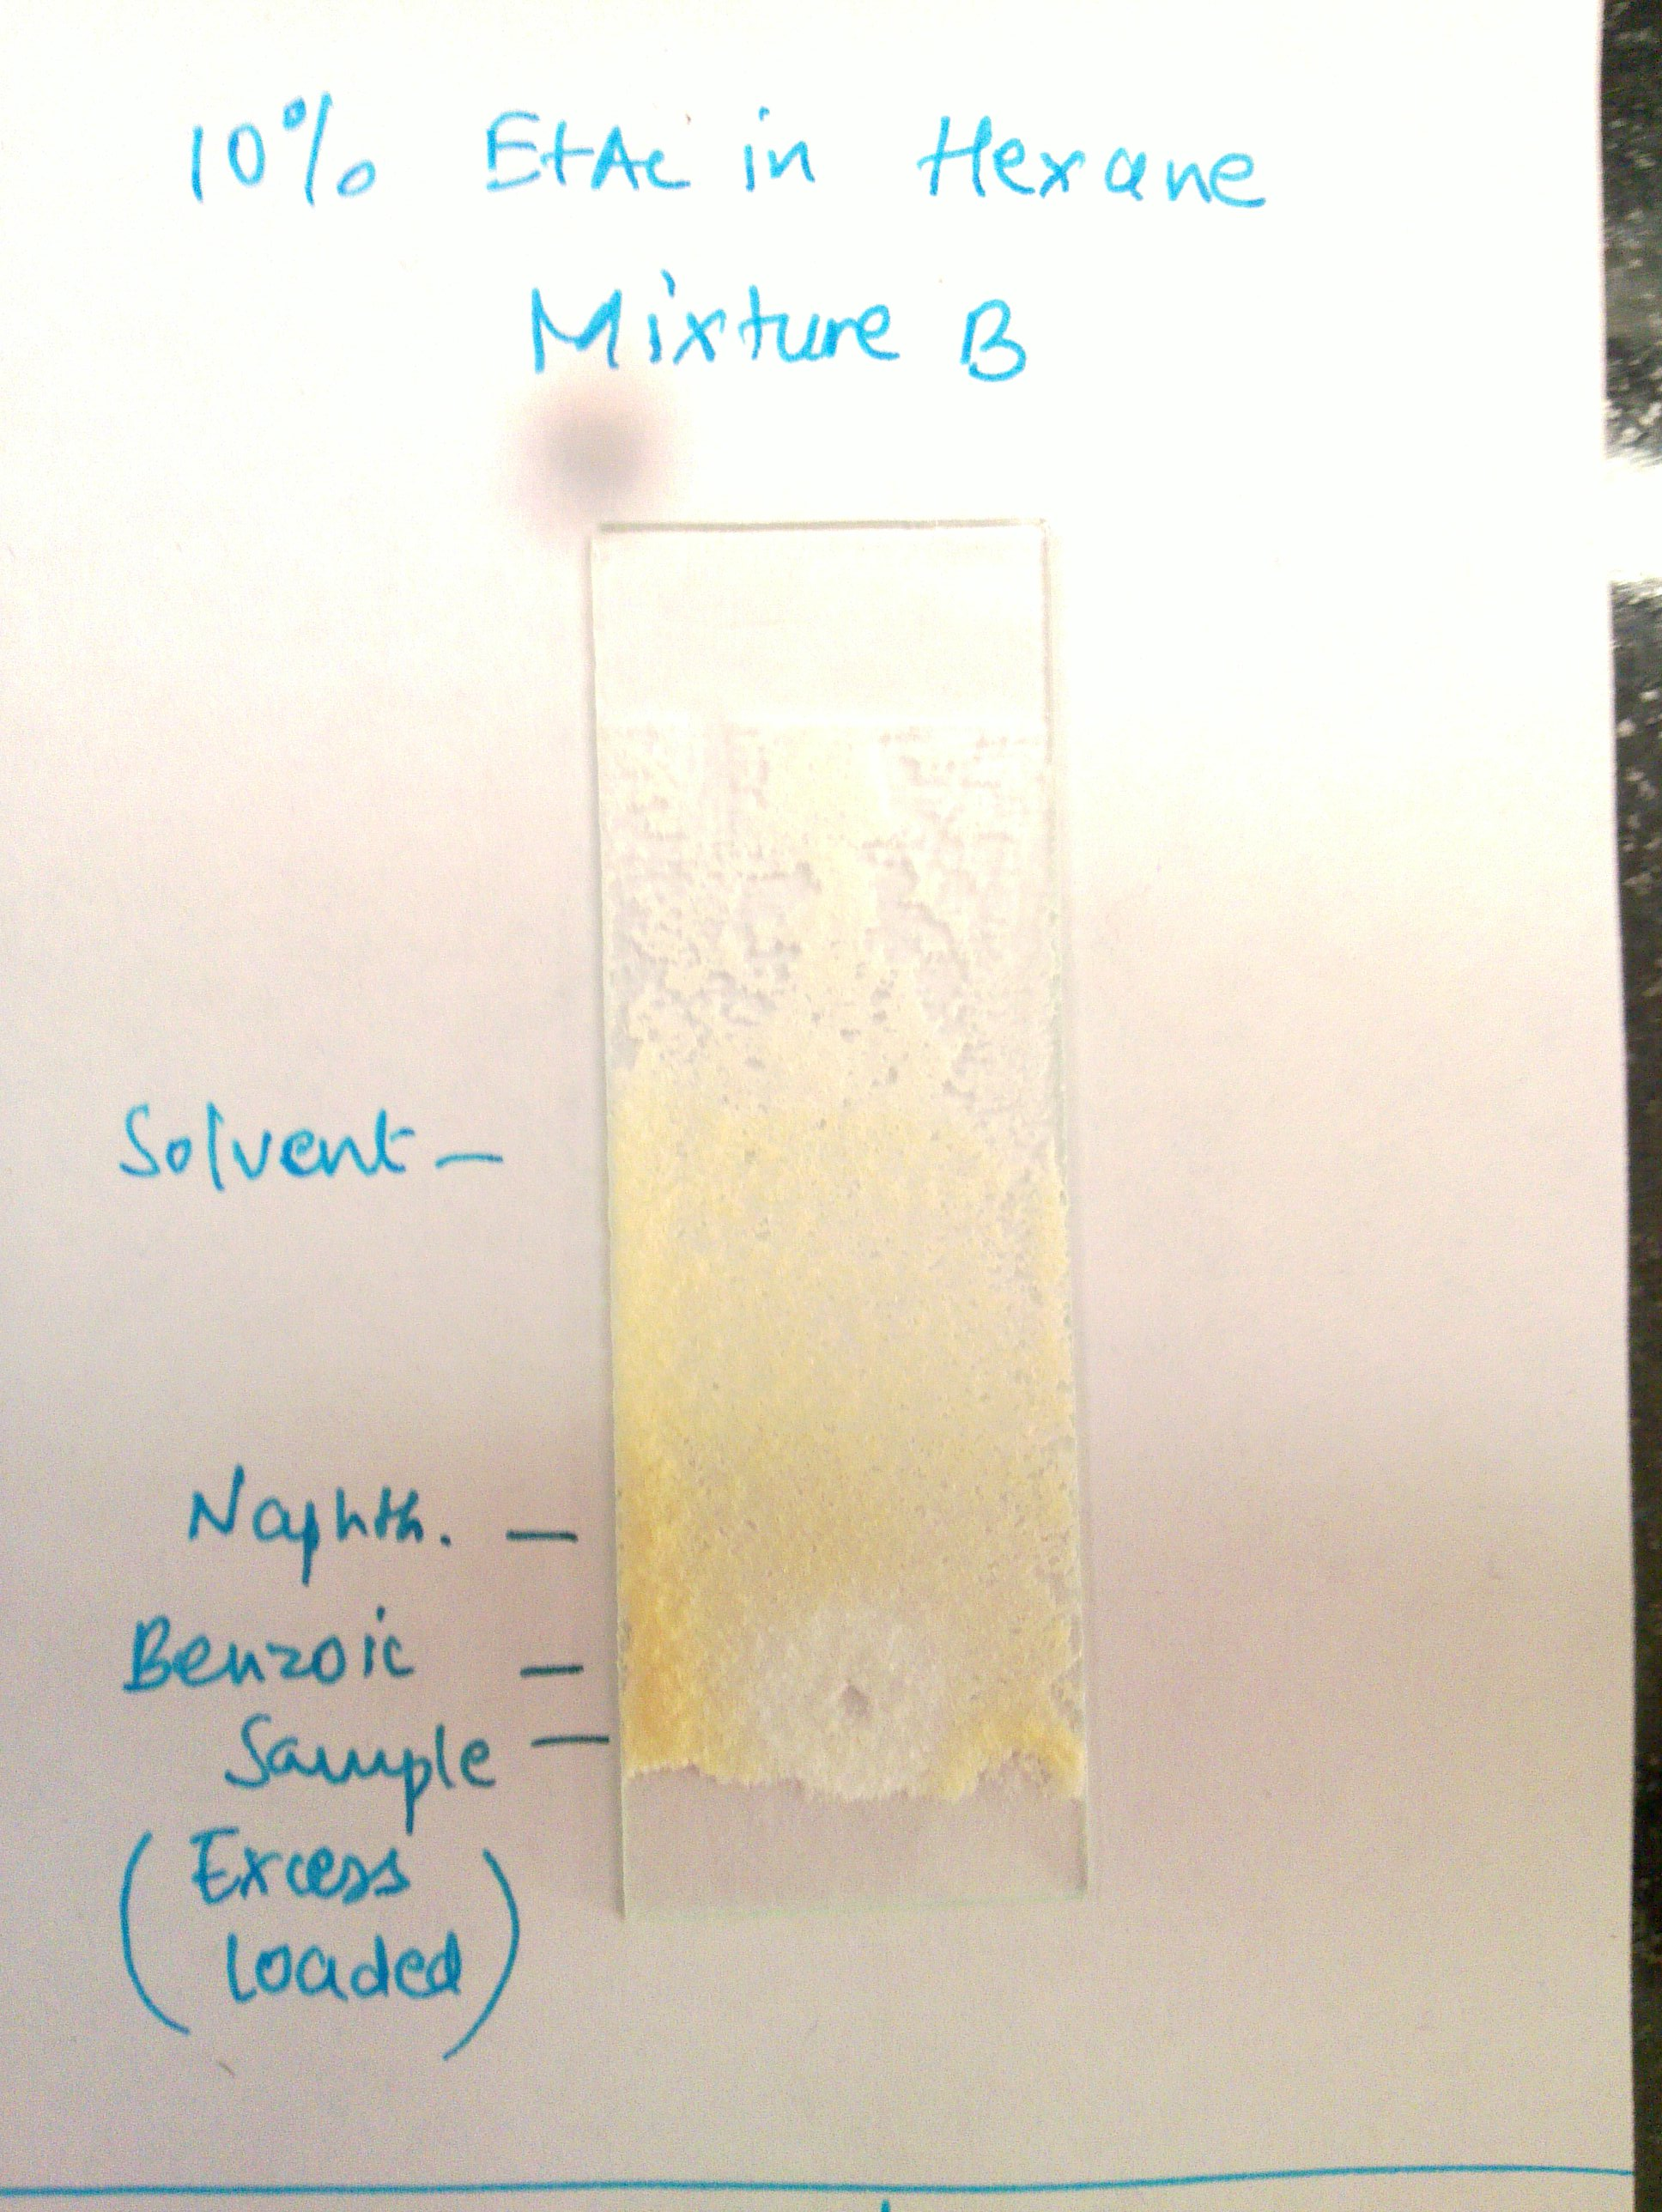
\includegraphics[width=0.4\linewidth]{gfx/e11_mixB}
		\end{center}
	\caption[TLC for Mixture 2]{Mixture 2} {\label{e11_mixB}}
	\end{figure}

	\begin{figure}[bth]
		\begin{center}
			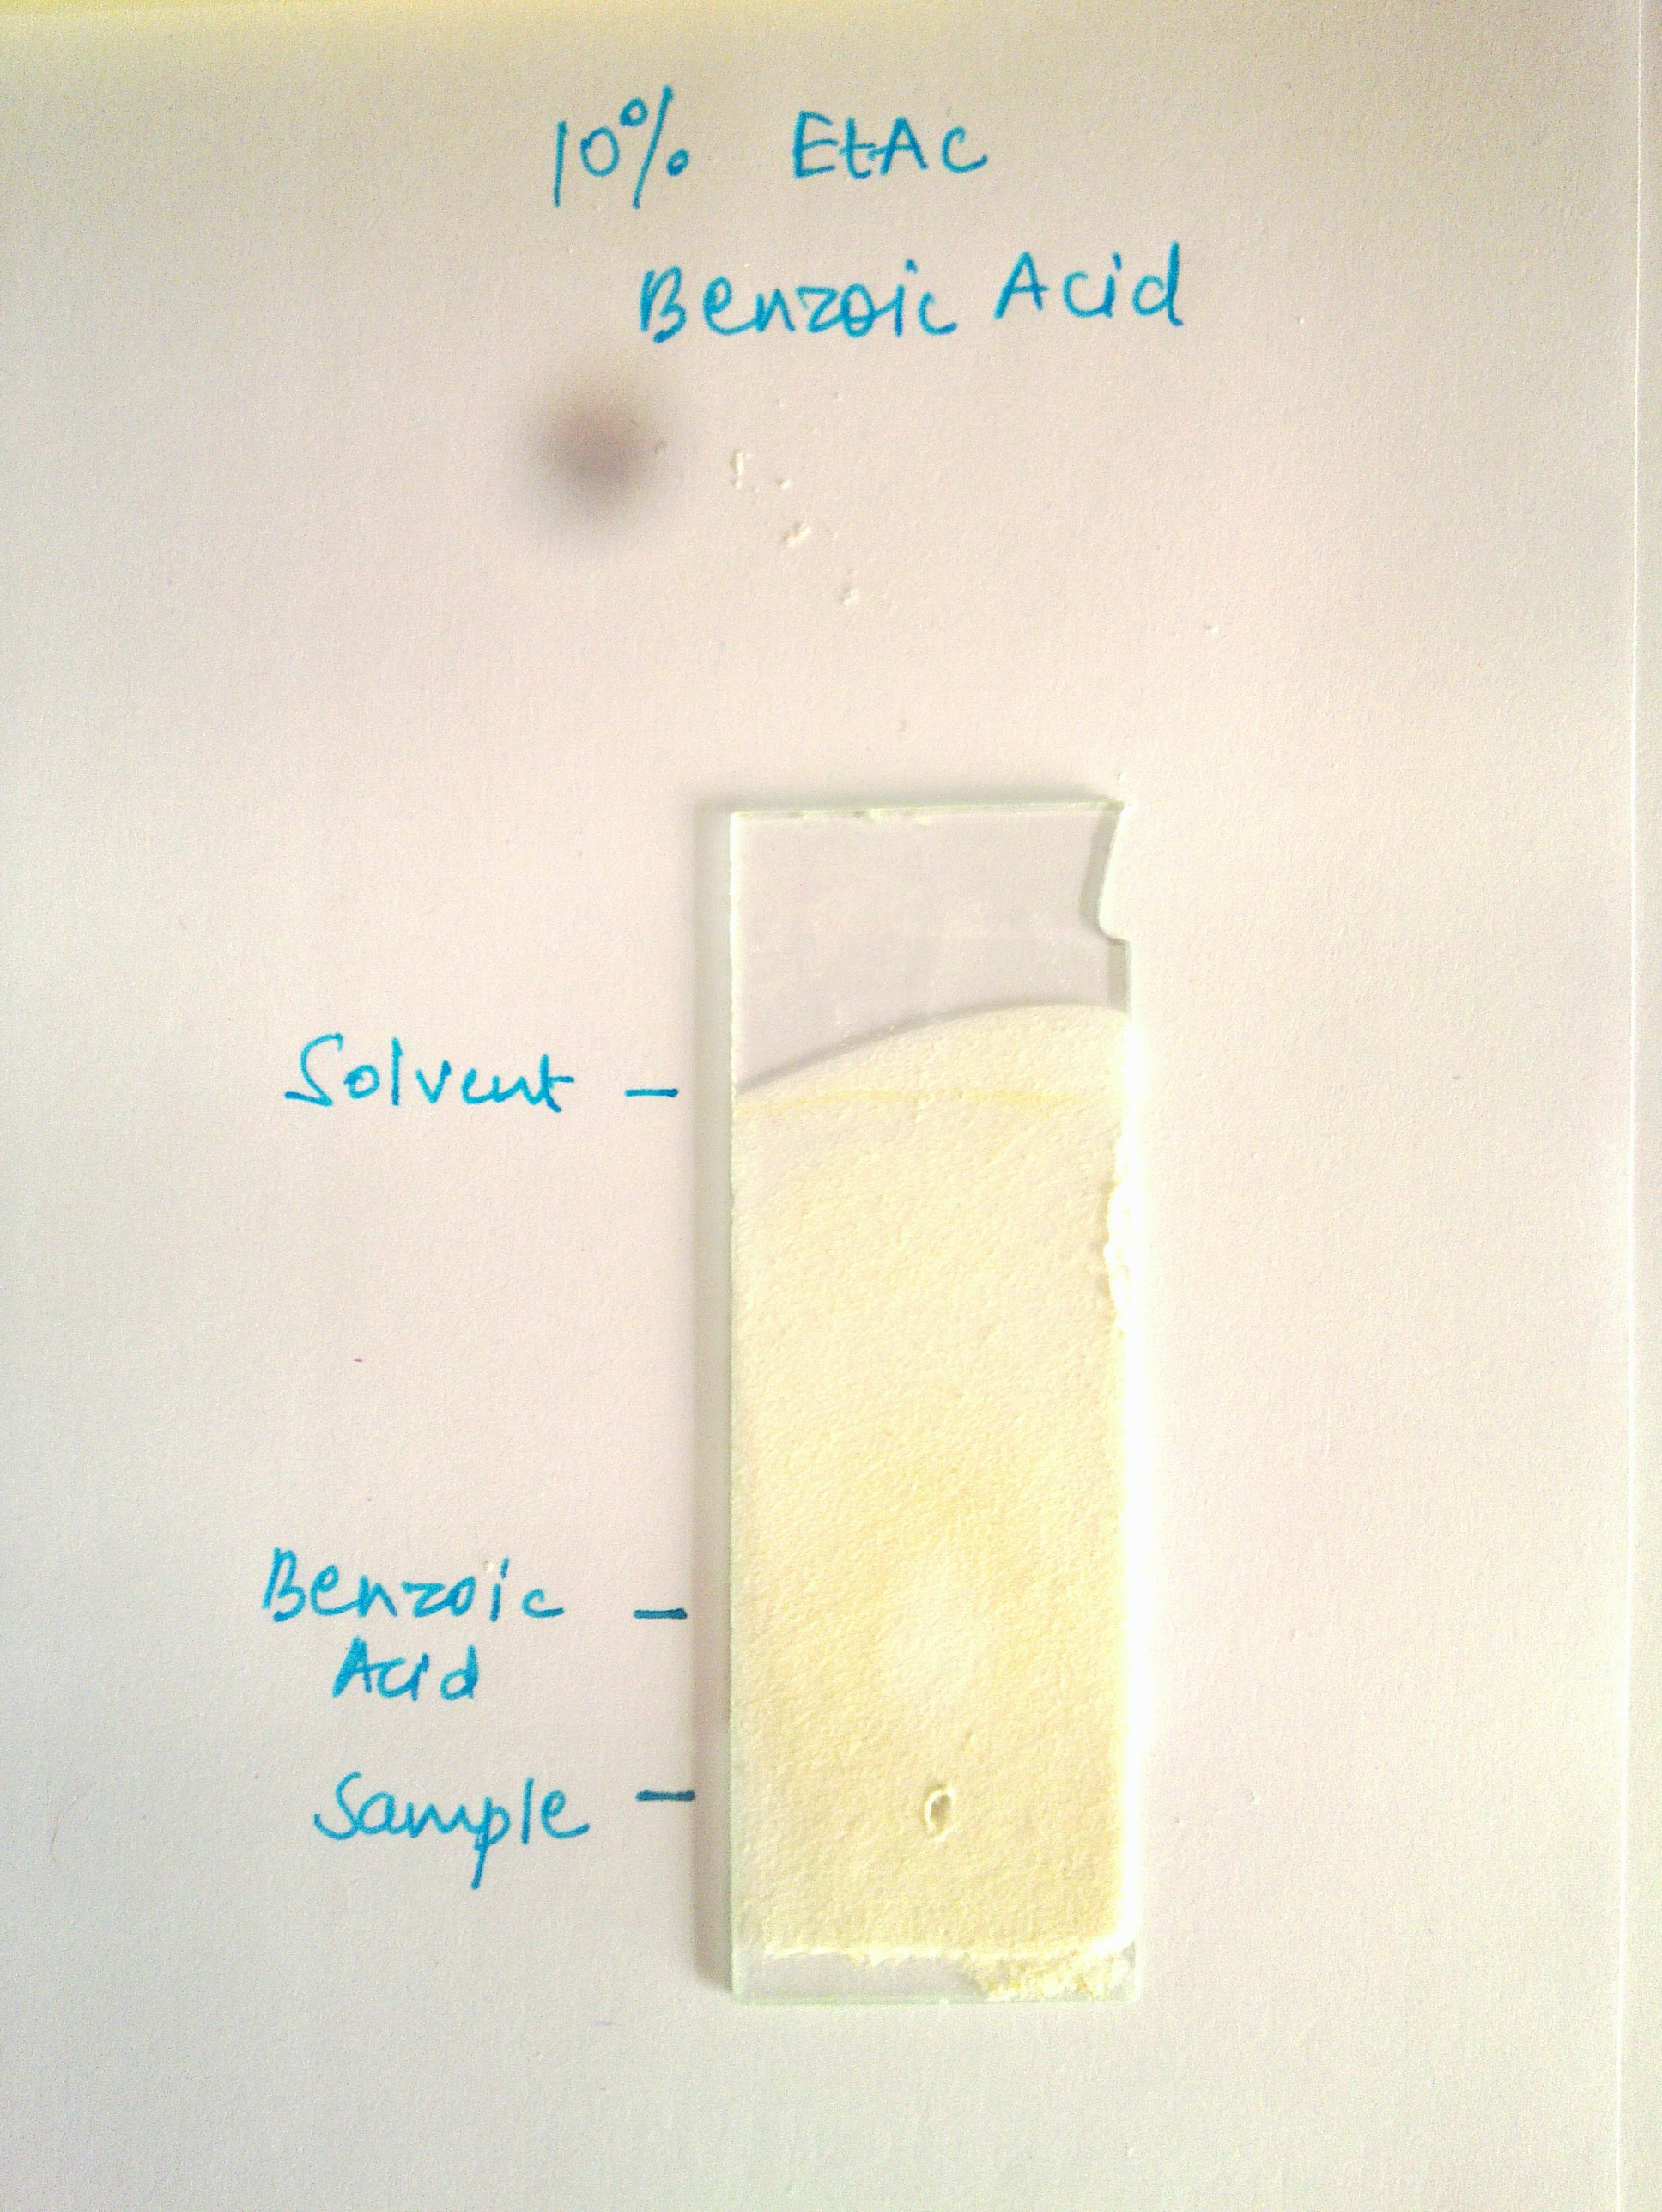
\includegraphics[width=0.4\linewidth]{gfx/e11_benzoic}
		\end{center}
	\caption[TLC for Benzoic Acid]{Benzoic Acid} {\label{e11_benzoic}}
	\end{figure}

	\begin{figure}[bth]
		\begin{center}
			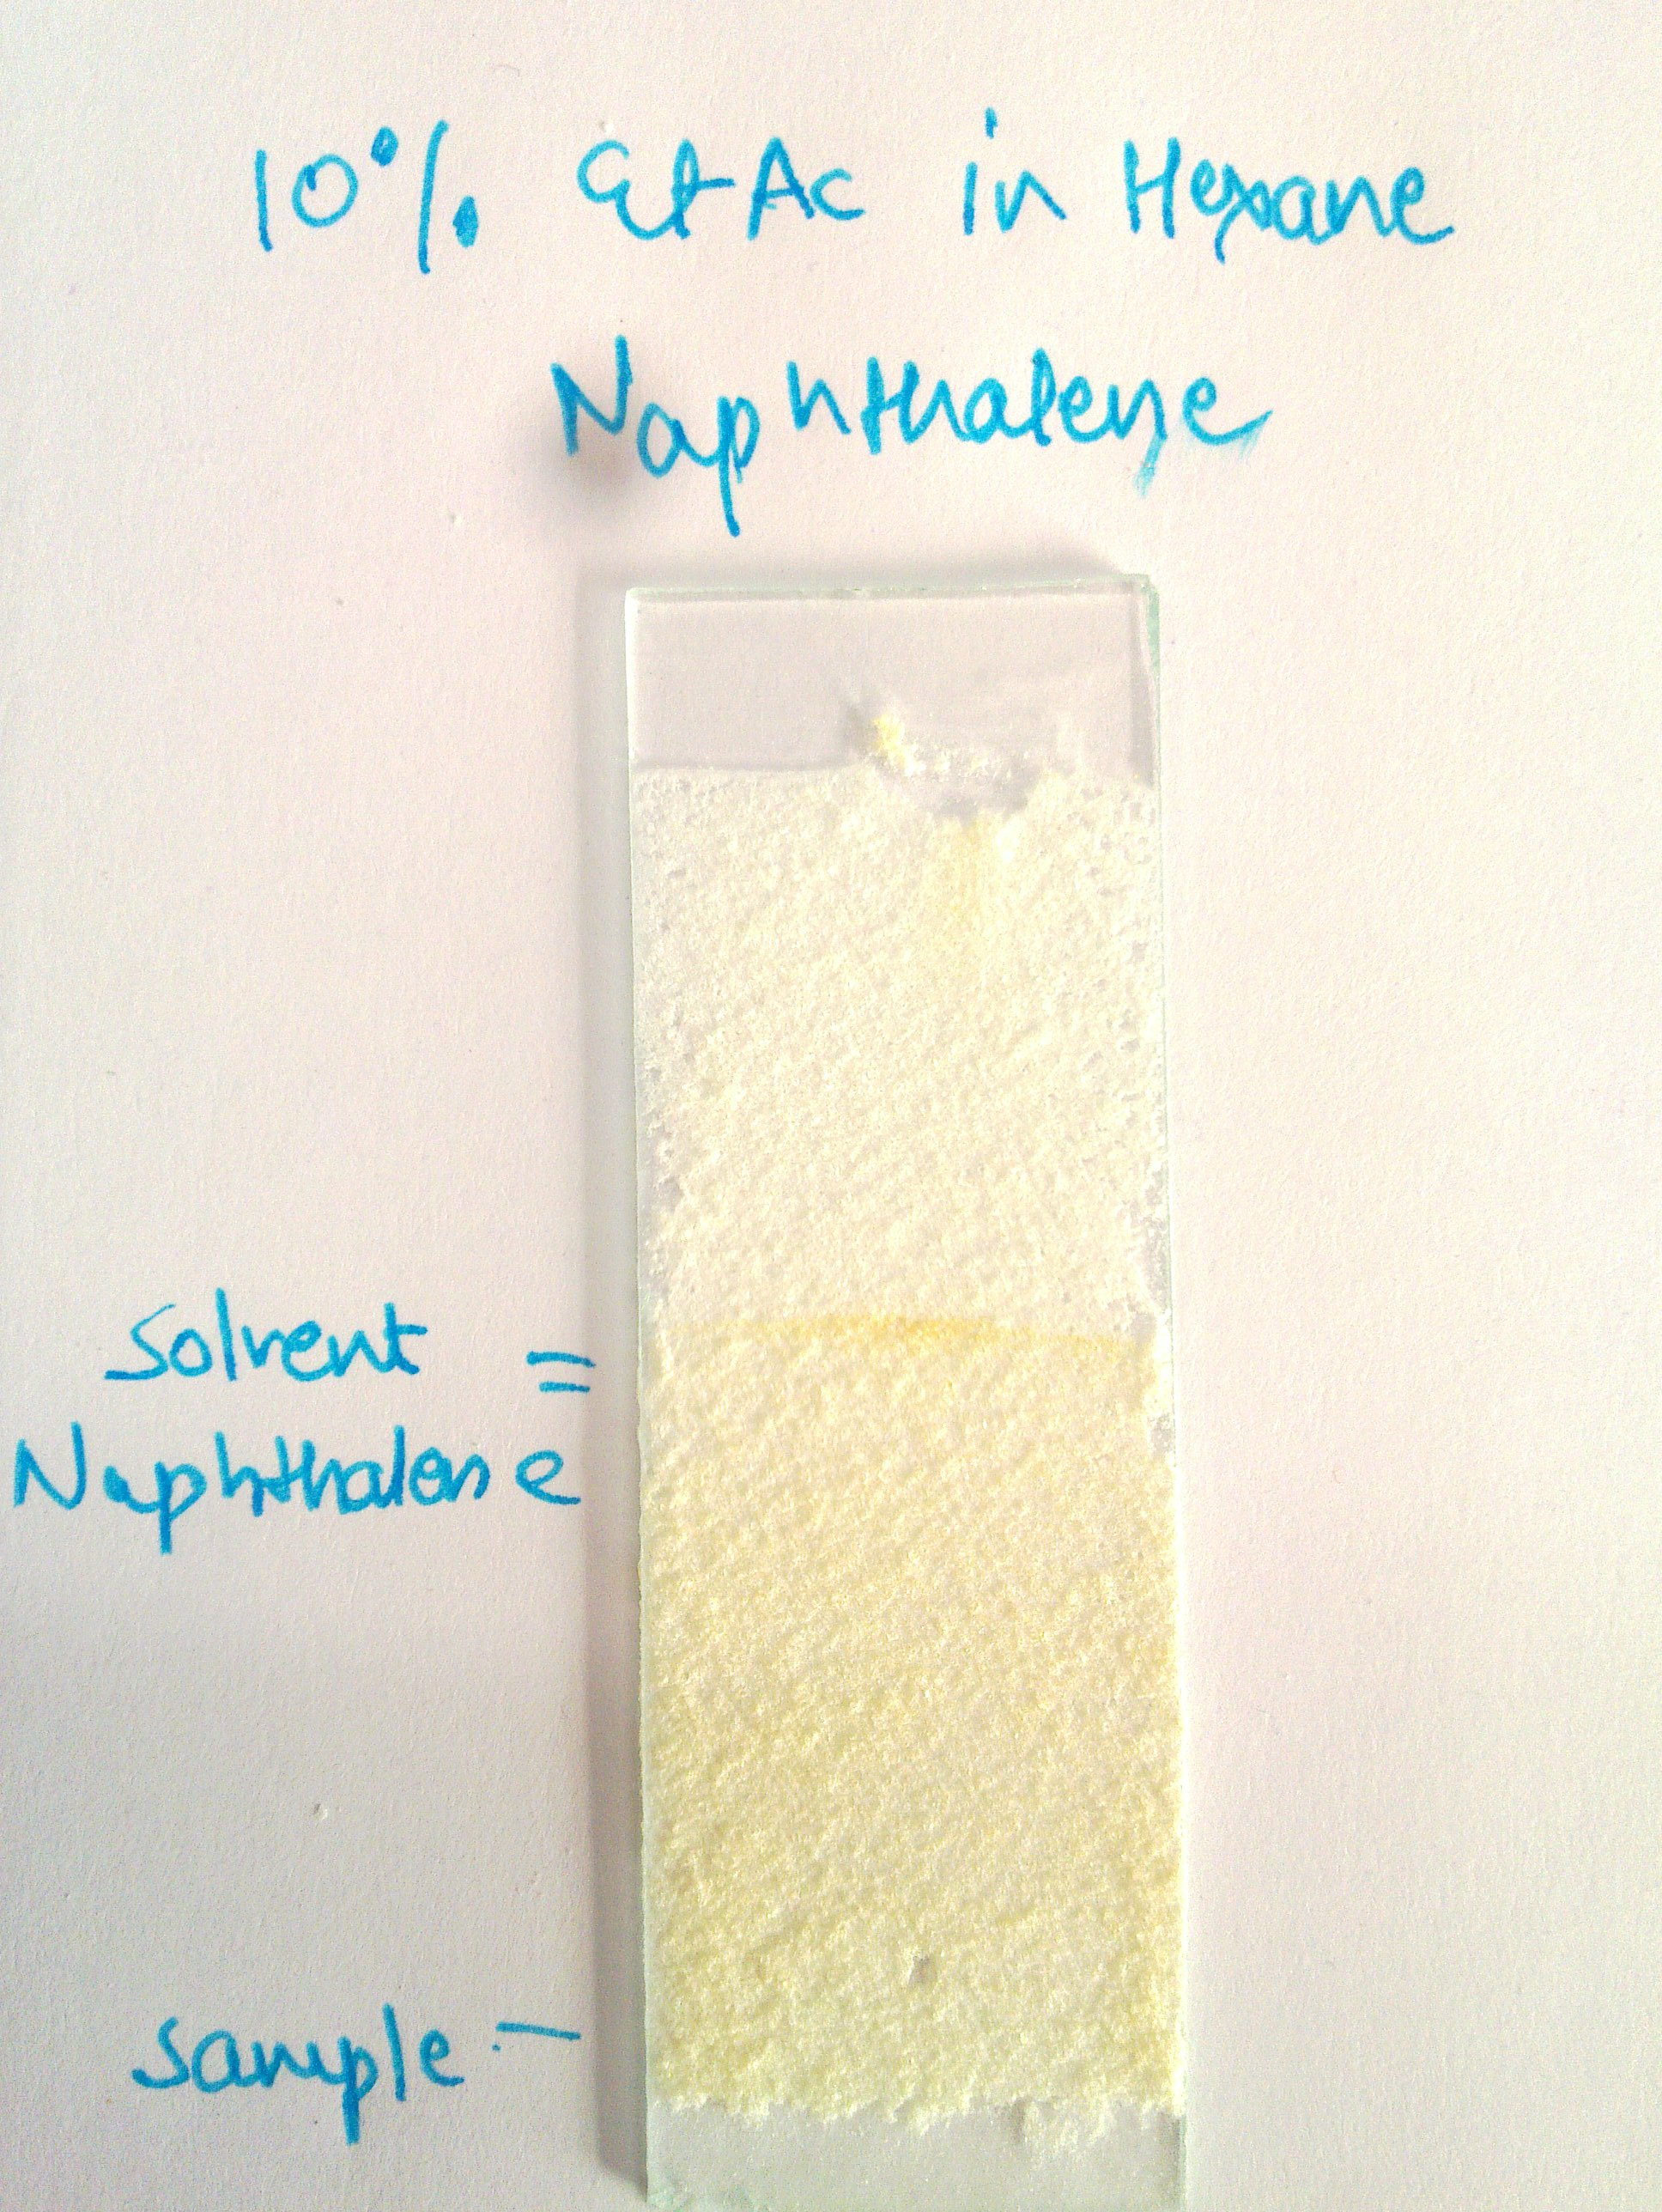
\includegraphics[width=0.4\linewidth]{gfx/e11_naphthalene}
		\end{center}
	\caption[TLC for Naphthalene]{Naphthalene} {\label{e11_naphthalene}}
	\end{figure}

\section{Precaution}
	Precautions are the similar to that given in \autoref{solventExtraction} viz.
	\begin{enumerate}
		\item The slurry shouldn't be very thick
		\item Cover the beakers with a watch glass to ensure there's no loss of volatile substances (minimal that is)
		\item The coating is very fragile, thus the TLC plates must be handled with caution
		\item Mixing should be done thoroughly to ensure proper extraction
		\item The nozzle of the separating funnel was handled carefully to extract the desired solution only
		\item A large volume of $NaHCO_3$ is required to neutralize $HCl$, so do not waste time with a dropper initially
		\item Neutralize, do not overshoot, although in this case it doesn't matter, but it might in some
	\end{enumerate}

	\marginpar{\Maggie We mistakenly started with 0.1 N HCl, which resulted in a disproportionate increase of volume of the extract}	
	
\section{Acknowledgements}
I thank Dr. R Vijaya Anand for his guidance during the experiment. I also acknowledge the contribution of my lab partners, Srijit, Prashansa and Vivek for performance of the same. I also thank our PhD guide for demonstrating the experiment and her assistance in general, with performance of the same.

	% \clearpage
	% \begin{figure}[bth]
	% 	\begin{center}
	% 		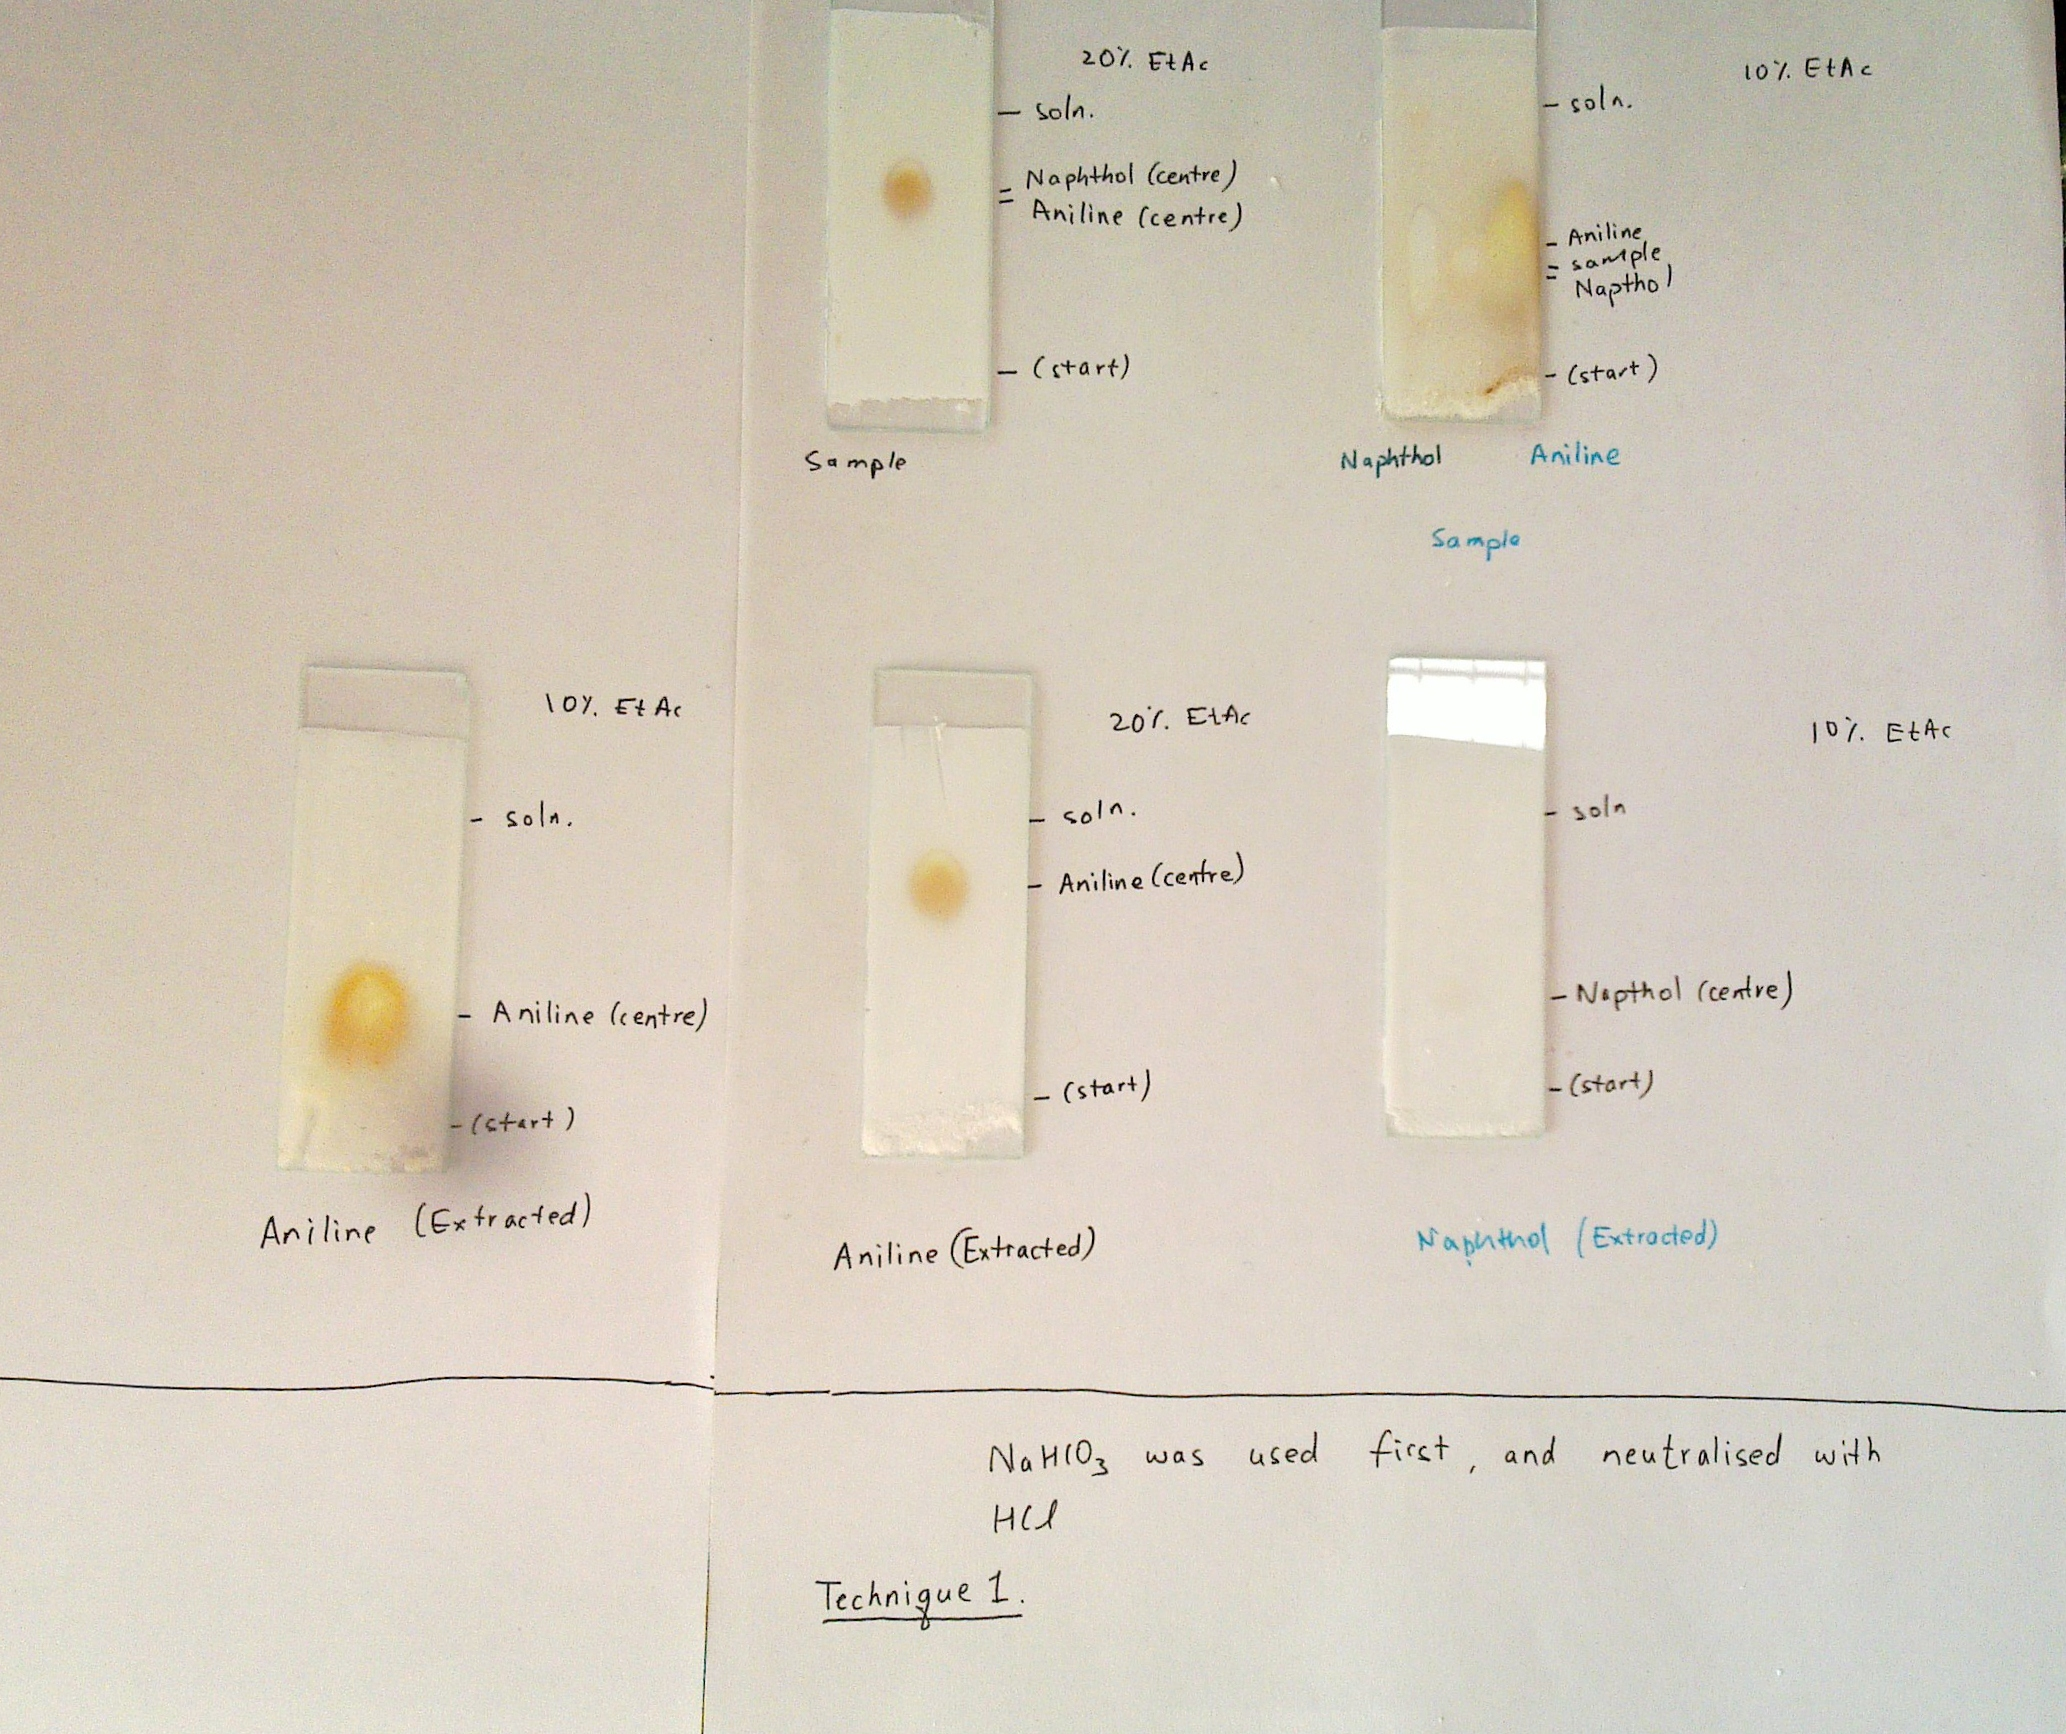
\includegraphics[width=1.5\linewidth]{gfx/e5_1}
	% 	\end{center}
	% \caption[TLCs Set 1]{\label{e5_1}}
	% \end{figure}

	% \begin{figure}[bth]
	% 	\begin{center}
	% 		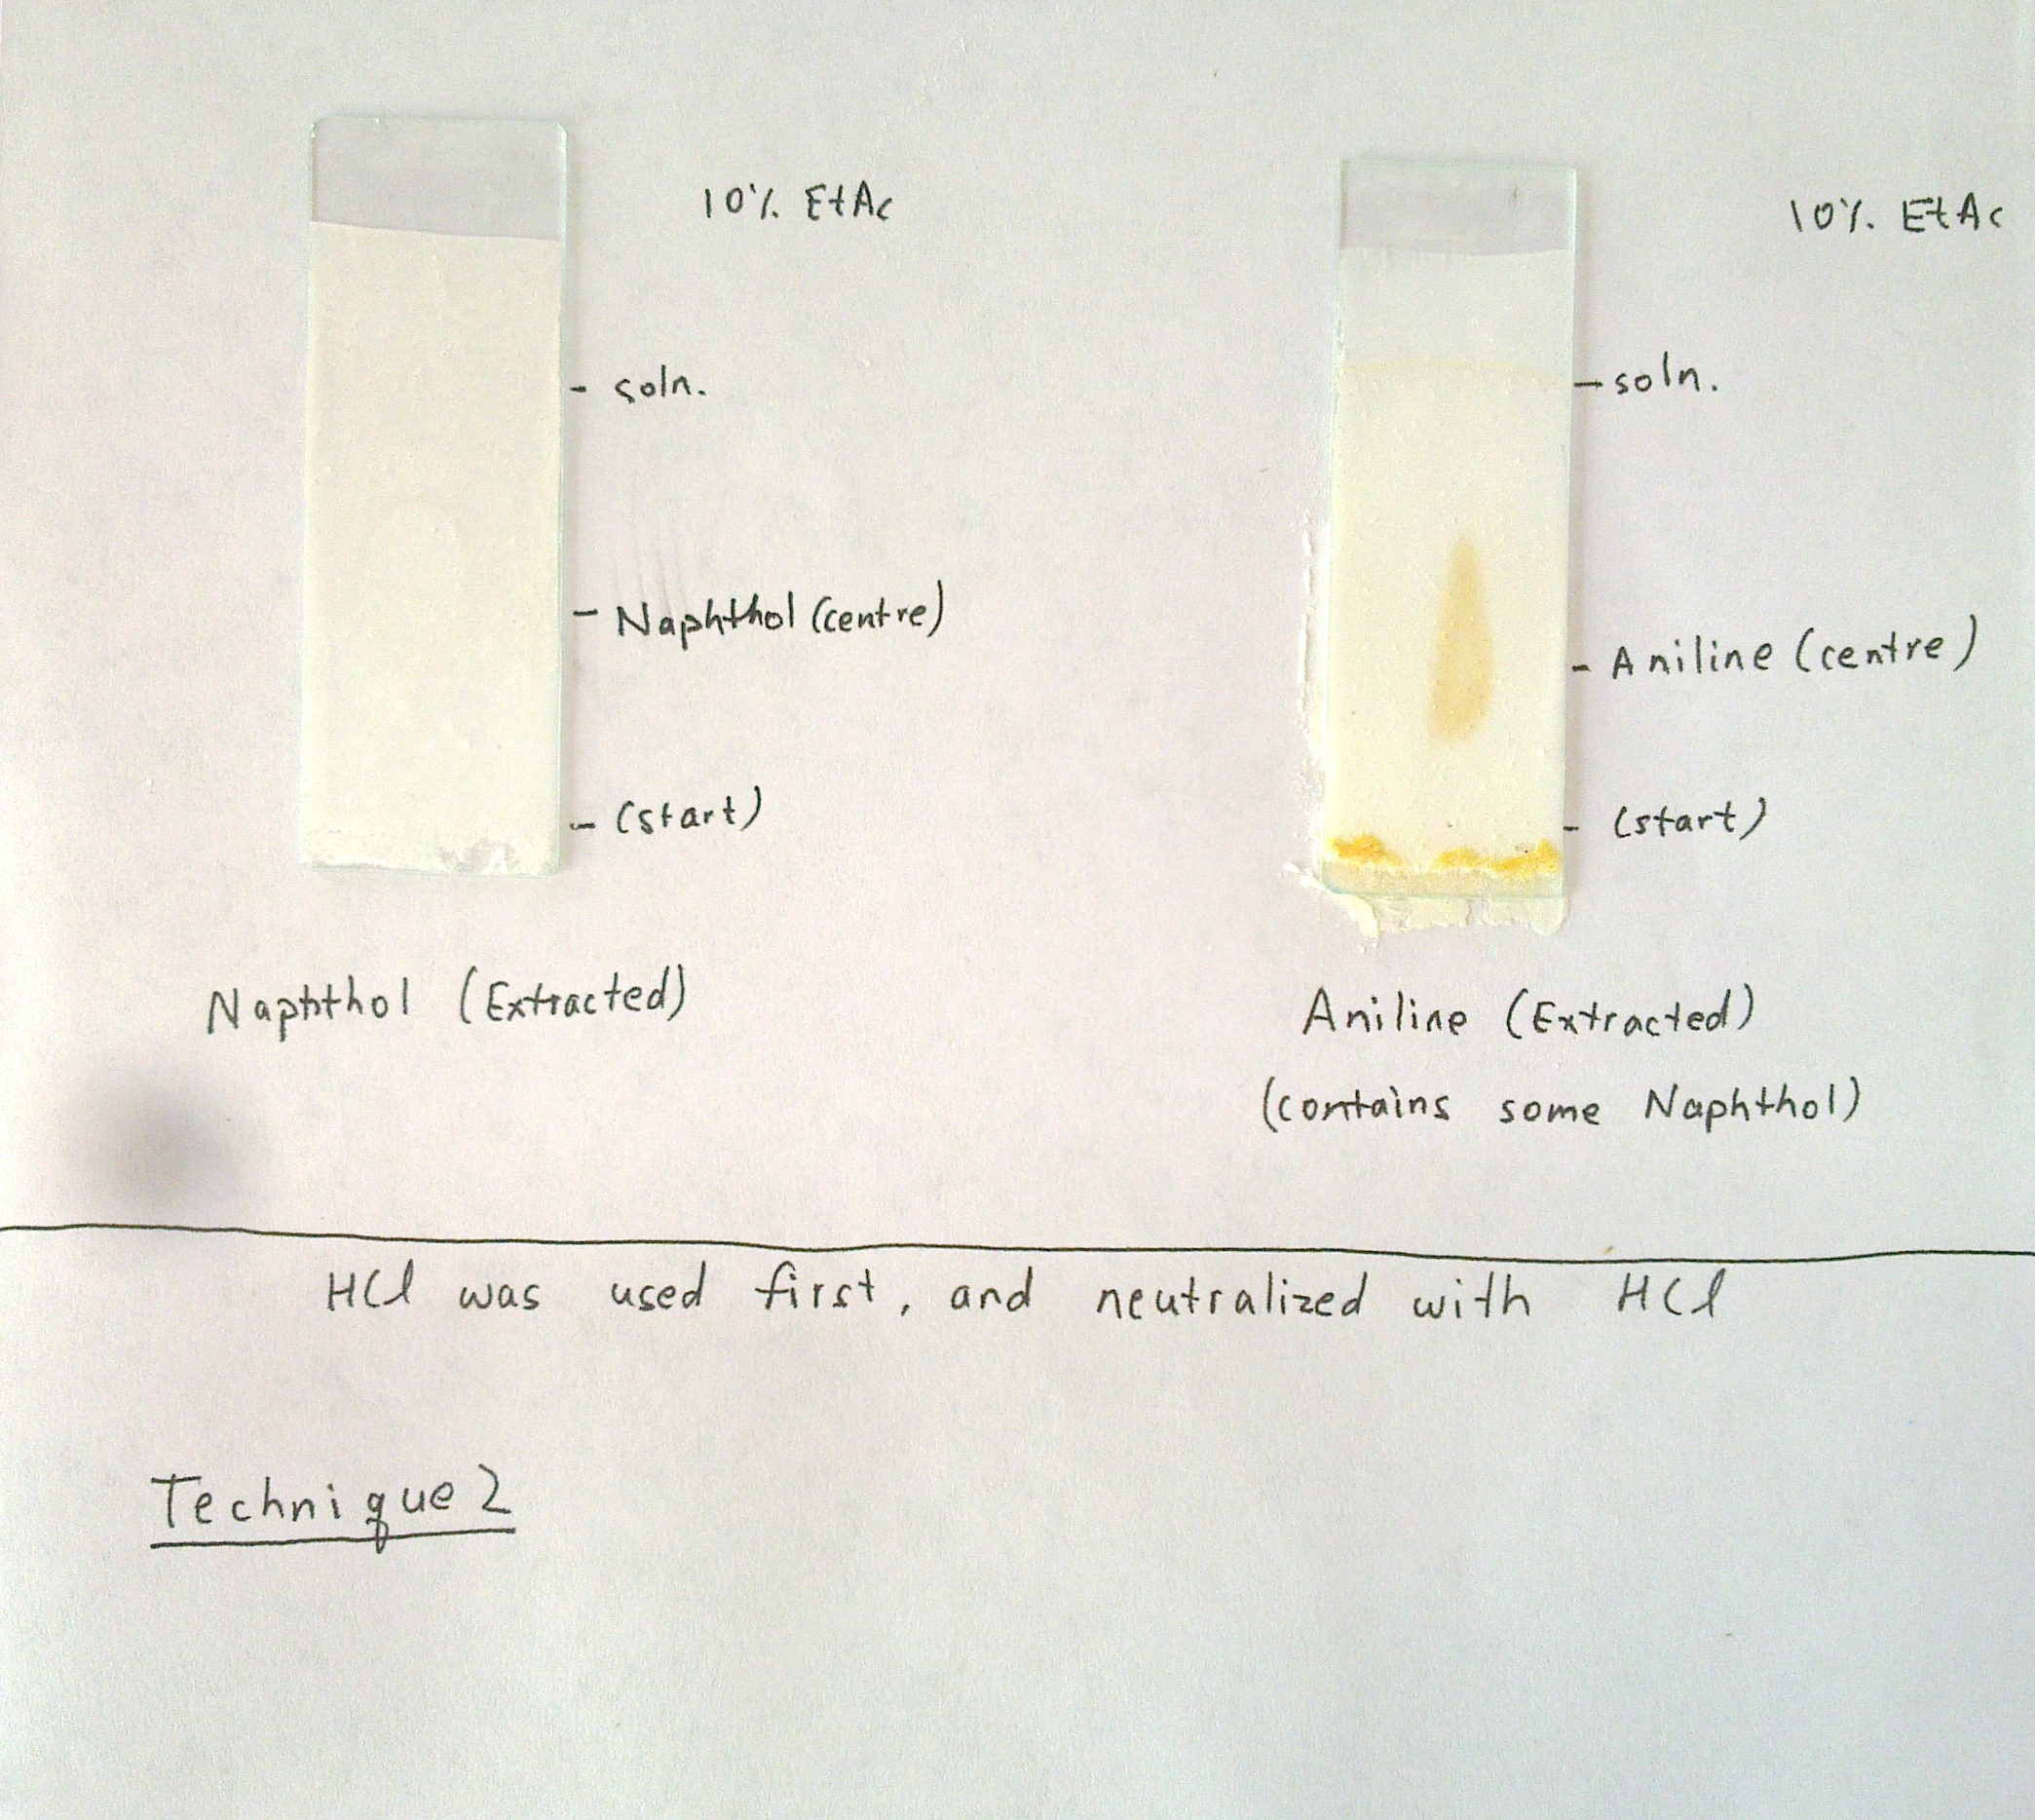
\includegraphics[width=1.0\linewidth]{gfx/e5_2}
	% 	\end{center}
	% \caption[TLCs Set 2]{\label{e5_2}}
	% \end{figure}